%%%%%%%%%%%%%%%%%%%%%%%%%%%%%%%%%%%%%%%%%%%%%%%%%%%%%%%%%%%%%%%%%%%%%%%%%%%

\documentclass[a4paper,oneside,12pt]{article}
\usepackage{mystyle}

\begin{document}

\title{\Large\bf Logarithmic functions}
\author{%%
  Minh Van Nguyen \\
  \url{mvngu@gmx.com}
}
\date{\today}
\maketitle


%%%%%%%%%%%%%%%%%%%%%%%%%%%%%%%%%%%%%%%%%%%%%%%%%%%%%%%%%%%%%%%%%%%%%%%%%%%

\section{What is logarithm?}

You already know that the function $f(x) = 10^x$ is an exponential
function.  Furthermore, the function $f(x)$ represents an exponential
growth.  Suppose you were to solve the equation
%%
\begin{equation}
\label{eqn:exponential_growth_100_10_x}
100
=
10^x
\end{equation}
%%
for $x$.  Take some time to think about what
\Equation{eqn:exponential_growth_100_10_x} is telling you.  The
equation tells you that you want a value of $x$ such that when $10$ is
raised to the power of $x$, you get $100$ as a result.  What would the
value of $x$ be?  Here, the number $10$ is the \emph{base} and the
unknown $x$ is the \emph{exponent}.  To solve
\Equation{eqn:exponential_growth_100_10_x} for $x$, take the logarithm
to base $10$ of both sides and you get
%%
\begin{equation}
\label{eqn:log10_100}
\log_{10} 100
=
\log_{10} (10^x).
\end{equation}
%%
The right-hand side of \Equation{eqn:log10_100} simplifies to
$\log_{10} (10^x) = x$ because the logarithm is to base $10$ and the
exponential function $10^x$ has base $10$.  In other words,
\Equation{eqn:log10_100} simplifies to
\[
\log_{10} 100
=
x.
\]
If $x = 2$, then $10^2 = 100$.  You say that $2$ is equivalent to the
logarithm of $100$ to base $10$.  In symbol, this is written as
\[
\log_{10}100
=
2.
\]
Thus the solution of \Equation{eqn:exponential_growth_100_10_x} is
$x = 2$.  The discussion is summarised in the next definition.

\begin{definition}
\textbf{Logarithm.}
Let $b$ and $y$ be positive numbers such that $b \neq 1$.  The
\emph{logarithm} to base $b$ of $y$ is equivalent to the exponent $x$
of $b$ such that $b^x = y$.  In symbols, you have $y = b^x$ if
$\log_b y = x$.
\end{definition}

The logarithm to base $10$ of $y > 0$ is written $\log_{10} y$ and is
called the \emph{common logarithm}.  If the base is $2$, then you
write $\log_2 y$, which is also called the \emph{binary logarithm}.
If the base is the irrational number $e$, you write $\log_e y$ and
call this the \emph{natural logarithm}.  Sometimes the natural
logarithm of $y$ is also written as $\ln y$.  Whenever you read about
or use logarithm, make sure that you know what base is used for the
logarithm.  Graphs of the above three logarithmic functions are
illustrated in \Figure{fig:logarithm:graphs}.  Note that
\Equation{eqn:log10_100} uses the common logarithm because the base is
$10$.  The right-hand side of \Equation{eqn:log10_100} simplifies to
$x$ due to \Theorem{thm:logarithm:lob_b_b_power_x} below.

\begin{figure}[!htbp]
\centering
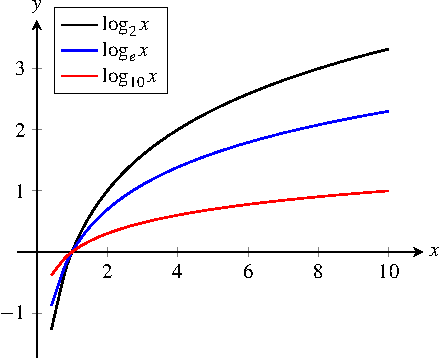
\includegraphics[scale=1.1]{image/12/logarithm.pdf}
\caption{%%
  Graphs of the binary logarithmic function $f(x) = \log_2 x$, the
  natural logarithmic function $f(x) = \log_e x$, and the common
  logarithmic function $f(x) = \log_{10} x$.
}
\label{fig:logarithm:graphs}
\end{figure}

\begin{example}
\textbf{Measuring acidity with pH.}
The pH of a liquid~(or aqueous solution) is a numerical value that is
used to classify whether the liquid is acidic, neutral, or
basic~(alkaline).\footnote{
  See page~670 of the book:
  R.~Chang and K.~A.~Goldsby. \emph{Chemistry}. $12$-th edition,
  McGraw-Hill Education, 2016.  Despite what some chemistry textbooks
  might tell you, a negative value of pH does exist; see the following
  paper: \url{https://doi.org/10.1021/ed083p1465}.
}
If $\molarH$ represents the molar concentration of hygrogen ions, then
the pH of $\molarH$ is defined as
%%
\begin{equation}
\label{eqn:logarithm:pH}
\text{pH}
=
-\log_{10} \molarH.
\end{equation}
%%
If an aqueous solution has a pH $< 7$, the solution is classified as
acidic.  If the solution has a pH $ = 7$, it is classified as
neutral.  An aqueous solution that has a pH $> 7$ is classified as
basic~(or alkaline).  A glass of lemon juice has a hydrogen ion
concentration of $5.4 \times 10^{-3}$
molar~(or $5.4 \times 10^{-3}$M).  Calculate the pH of the lemon juice
and classify its acidity.
\end{example}

\begin{solution}
You have $\molarH = 5.4 \times 10^{-3}$M.  Substitute the number into
\Equation{eqn:logarithm:pH} and you get
%%
\begin{align*}
\text{pH}
&=
-\log_{10} (5.4 \times 10^{-3}) \\[4pt]
&\approx
2.3
\end{align*}
%%
rounded to one decimal place.  Since the pH of the lemon juice is less
than $7$, the lemon juice is classified as acidic.
\end{solution}

\begin{exercise}
\textbf{The pH of blood.}
A specimen of blood has a hydrogen ion concentration of
$4 \times 10^{-8}$M.  Calculate the pH of the specimen and classify
its acidity.
\end{exercise}

\ifbool{showSolution}{
\begin{solution}
Substitute the expression $\molarH = 4 \times 10^{-8}$M into
\Equation{eqn:logarithm:pH} and you have
%%
\begin{align*}
\text{pH}
&=
-\log_{10} (4 \times 10^{-8}) \\[4pt]
&\approx
7.4
\end{align*}
%%
rounded to one decimal place.  As the pH of the blood specimen is
greater than $7$, the specimen is classified as basic.
\end{solution}
}{}

\begin{theorem}
\label{thm:logarithm:lob_b_b_power_x}
Let $b > 0$ be any real number such that $b \neq 1$ and let $x$ be a
real variable.  Then $\log_b (b^x) = x$.
\end{theorem}

Why is \Theorem{thm:logarithm:lob_b_b_power_x} important?
\Theorem{thm:logarithm:lob_b_b_power_x} is often used to solve
equations that involve exponential functions.  In fact, you have
already seen how the theorem was used to solve
\Equation{eqn:exponential_growth_100_10_x} for $x$.  Here are some
more examples.

\begin{example}
Solve the equation $2^x = 64$ for $x$.
\end{example}

\begin{solution}
The equation $2^x = 64$ asks for a value of $x$ such that when $2$ is
raised to the power of $x$, the result will be $64$.  Since the base
is $2$, take the logarithm to base $2$ of both sides of the equation
and you get $\log_2(2^x) = \log_2 64$.  Use
\Theorem{thm:logarithm:lob_b_b_power_x} to simplify the left-hand side
as $\log_2(2^x) = x$, hence you can write $x = \log_2 64$.  You can
use a calculator or computer program to determine that
$x = \log_2 64 = 6$.  As a check, you can see that $2^6 = 64$.
\end{solution}

\begin{example}
\textbf{Population of Australia.}
According to the Australian Bureau of Statistics~(ABS), at the end of
September 2017 the population of Australia grew by $1.6\%$ since the
previous year.\footnote{
  ``3101.0 - Australian Demographic Statistics, Sep 2017'',
  \url{http://web.archive.org/web/20180420062713/http://www.abs.gov.au/AUSSTATS/abs@.nsf/Lookup/3101.0Main+Features1Sep\%202017},
  accessed 2018-04-20.
}
The population by the end of the given period was estimated to be
$24.7029$ million people.  Assume that for the next few years the
population of Australia will grow by a constant rate of $1.6\%$ per
annum.  When will the population of Australia be $30$ million people?
\end{example}

\begin{solution}
You have seen this example before and know that the population~(in
millions) in $t$ years from $2017$ onwards can be written as
\[
P(t)
=
24.7029 \times 1.016^t.
\]
Note that the base is $b = 1.016$.  You want to determine the number
of years $t$ such that $P(t) = 30$ million people.  In other words,
you want to solve the equation
\[
30
=
24.7029 \times 1.016^t
\]
for $t$.  Divide both sides by $24.7029$ to get
$\frac{30}{24.7029} = 1.016^t$.  Now take the logarithm to base
$b = 1.016$ of both sides and you end up with
\[
\log_{1.016} \frac{30}{24.7029}
=
\log_{1.016} (1.016^t).
\]
Use \Theorem{thm:logarithm:lob_b_b_power_x} to simplify the right-hand
side to $\log_{1.016} (1.016^t) = t$ and you can now write
%%
\begin{equation}
\label{eqn:logarithm:Australia_population_doubling_time}
\log_{1.016} \frac{30}{24.7029}
=
t.
\end{equation}
%%
The latter expression evaluates to approximately $t \approx 12.2392$,
rounded to four decimal places.  As a check, you can see that in
approximately $t = 12.2392$ years the population of Australia will be
\[
24.7029 \times 1.016^{12.2392}
\approx
30.000011
\]
million people, rounded to six decimal places.  Therefore some time in
the year $2017 + 12 = 2029$ the population of Australia will be
approximately $30$ million people.
\end{solution}

\begin{exercise}
\textbf{Bacterial growth.}
A Petri dish initially contains ten cells of a type of bacteria.  The
bacteria population is known to have a constant percentage growth rate
of $56\%$ per hour.
%%
\begin{packedenum}
\item\label{subex:logarithm:bacterial_growth_at_least_100_cells}
  Use logarithm to calculate the amount of time required for the
  bacteria population to be at least $100$ cells.

\item\label{subex:logarithm:bacterial_growth_doubling_time}
  Use logarithm to calculate the doubling time of the bacteria
  population.
\end{packedenum}
\end{exercise}

\ifbool{showSolution}{
\begin{solution}
\solutionpart{subex:logarithm:bacterial_growth_at_least_100_cells}
From a previous example, you know that the bacteria population can be
written as $Q(t) = 10 \times 1.56^t$.  Now you want to solve the
equation
\[
100
=
10 \times 1.56^t
\]
for $t$.  Divide both sides of the latter equation by $10$ to get
$\frac{100}{10} = 1.56^t$, which simplifies to $10 = 1.56^t$.  In the
exponential function $1.56^t$, the base is $b = 1.56$.  Take the
logarithm to base $b = 1.56$ of both sides of $10 = 1.56^t$ and you
end up with $\log_{1.56} 10 = \log_{1.56} (1.56^t)$, which by
\Theorem{thm:logarithm:lob_b_b_power_x} can be simplified as
$\log_{1.56} 10 = t$.  Thus $t$ is approximately $t \approx 5.1780$,
rounded to four decimal places.  As a check, note that
$Q(5.1780) = 10 \times 1.56^{5.1780} \approx 99.9998$, rounded to four
decimal places.  However, if $t = 5.1781$ then you have
$Q(5.1781) = 10 \times 1.56^{5.1781} \approx 100.0043$, rounded to
four decimal places.  In other words, you must wait a minimum of
$5.1781$ hours in order for the bacteria population to be at least
$100$ cells.

\solutionpart{subex:logarithm:bacterial_growth_doubling_time}
The initial bacteria population is $a = 10$ cells.  Double this and
you get $2a = 2 \times 10 = 20$ cells.  You want to know the amount of
time required in order for the bacteria population to double from $10$
cells to $20$ cells.  That is, you want to solve the equation
\[
20
=
10 \times 1.56^t
\]
for $t$.  Divide both sides of the latter equation by $10$ to get
$\frac{20}{10} = 1.56^t$, which simplifies to $2 = 1.56^t$.  Taking
the logarithm to base $b = 1.56$ of both sides yields
$\log_{1.56} 2 = \log_{1.56} (1.56^t)$ and use
\Theorem{thm:logarithm:lob_b_b_power_x} to simplify the last equation
to $\log_{1.56} 2 = t$.  Then $t$ is approximately
$t \approx 1.5587$, rounded to four decimal places.  As a check, you
have $Q(1.5587) = 10 \times 1.56^{1.5587} \approx 19.9997$, rounded to
four decimal places.  However, if $t = 1.5588$ then you get
$Q(1.5588) = 10 \times 1.56^{1.5588} \approx 20.0006$, rounded to four
decimal places.  Conclude that the doubling time of the bacteria
population is approximately $1.5588$ hours.
\end{solution}
}{}

\begin{example}
\textbf{Radiocarbon dating.}
Carbon-$14$ decays at a rate of approximately $r = 0.00012097$ per
annum, rounded to eight decimal places.  Calculate the half-life of
$300$ isotopes of carbon-$14$.
\end{example}

\begin{solution}
Radioactive decay follows an exponential decay model of the form
\[
A(t)
=
a e^{-rt}.
\]
Here, $a$ represents the initial number of radioactive isotopes,
$r > 0$ denotes the decay rate as a decimal, and $A(t)$ represents the
remaining number of radioactive isotopes after $t$ units of time.  In
the example, you initially have $a = 300$ isotopes of carbon-$14$ and
the decay rate is $r = 0.00012097$ per annum.  After $t$ years, the
number of remaining carbon-$14$ isotopes can be written as
\[
A(t)
=
300 e^{-0.00012097 t}.
\]
You want to know the number of years required for the initial $300$
isotopes to decay to $\frac{300}{2} = 150$ isotopes.  That is, you
want to solve the equation
\[
150
=
300 e^{-0.00012097 t}
\]
for $t$.  Divide both sides by $300$ to get
$\frac{150}{300} = e^{-0.00012097 t}$, which simplifies to
$\frac{1}{2} = e^{-0.00012097 t}$.  In the exponential function
$e^{-0.00012097 t}$, the base is the irrational number $e$.  Take the
logarithm to base $e$ of both sides of
$\frac{1}{2} = e^{-0.00012097 t}$ and you end up with
$\ln \bigparen{\frac{1}{2}} = \ln \bigparen{e^{-0.00012097 t}}$,
which by \Theorem{thm:logarithm:lob_b_b_power_x} simplifies to
$\ln \bigparen{\frac{1}{2}} = -0.00012097 t$.  Solving the latter
equation for $t$ yields
\[
-\frac{1}{0.00012097}
\ln \parenthesis*{\frac{1}{2}}
=
t
\]
which evaluates to approximately $t \approx 5730$ years, rounded to
the nearest integer.  Conclude that the initial $300$ carbon-$14$
isotopes have a half-life of approximately $5730$ years.
\end{solution}

\begin{exercise}
\textbf{Fermium-$250$.}
Fermium-$250$ is known to have a decay rate of approximately $0.0231$
per minute.  Calculate the half-life of $100$ isotopes of
fermium-$250$.
\end{exercise}

\ifbool{showSolution}{
\begin{solution}
If $A(t)$ represents the number of remaining fermium-$250$ isotopes
after $t$ minutes, then $A(t)$ can be written as
\[
A(t)
=
100 e^{-0.0231 t}.
\]
Half of $100$ is $100 / 2 = 50$ and you want to solve the equation
\[
50
=
100 e^{-0.0231 t}
\]
for $t$.  In the latter equation, divide both sides by $100$ to get
$\frac{50}{100} = e^{-0.0231 t}$, which simplifies to
$\frac{1}{2} = e^{-0.0231 t}$.  Take the logarithm to base $e$ of both
sides and you end up with
$\ln \parenthesis*{\frac{1}{2}} = \ln \parenthesis*{e^{-0.0231 t}}$,
which by \Theorem{thm:logarithm:lob_b_b_power_x} simplifies to
$\ln \parenthesis*{\frac{1}{2}} = -0.0231 t$.  The last equation
can be solved for $t$ to get
\[
t
=
-\frac{1}{0.0231}
\ln \parenthesis*{\frac{1}{2}}
\]
which evaluates to approximately $t \approx 30$, rounded to the
nearest integer.  Therefore the half-life of $100$ isotopes of
fermium-$250$ is approximately $30$ minutes.
\end{solution}
}{}


%%%%%%%%%%%%%%%%%%%%%%%%%%%%%%%%%%%%%%%%%%%%%%%%%%%%%%%%%%%%%%%%%%%%%%%%%%%

\section{Properties of logarithm}

One of the most useful properties of logarithm is that exponentiation
and logarithm are inverse functions of each other.  This is similar to
the way addition and subtraction are inverse operations of each other,
or multiplication and division are inverse operations of each other.
Consequently, you can use this inverse property between exponentiation
and logarithm to solve equations that involve exponential and
logarithmic functions.  What does all this mean?

Consider the example of addition and subtraction.  Suppose you have
two numbers $a$ and $x$ such that $a \neq 0$.  Adding $a$ to $x$
results in $x + a$.  You can undo the addition by subtracting $a$ from
$x + a$.  Doing so gives you the expression
\[
(x + a) - a
=
x + a - a
=
x.
\]
On the other hand, suppose you subtract $a$ from $x$ and end up with
$x - a$.  Undoing the subtraction requires that you add $a$ to
$x - a$.  Doing so results in
\[
(x - a) + a
=
x - a + a
=
x.
\]
The core idea is that addition and subtraction are inverse operations
of each other.  This inverse property between addition and subtraction
allows you to undo the result of any of the two operations.

As another example, consider multiplication and division.  Let $a$ and
$x$ be any numbers such that $a \neq 0$ and $x \neq 0$.  Multiplying
$x$ by $a$ results in $ax$.  To undo the multiplication, you divide
$ax$ by $a$ to produce
\[
\frac{ax}{a}
=
\frac{a}{a} \times x
=
x.
\]
On the other hand, suppose that you divide $x$ by $a$ to get $x / a$.
To undo the division, you multiply $x / a$ by $a$ to get
\[
\frac{x}{a} \times a
=
\frac{a}{a} \times x
=
x.
\]
Thus you see that multiplication and division are inverse operations
of each other.  This inverse property between multiplication and
division allows you to undo the result of any of the two operations.

The fact that exponentiation and logarithm are inverses of each other
is summarised in \Theorem{thm:logarithm:lob_b_b_power_x}.  This
inverse property between exponentiation and logarithm can be
visualised as the graph shown in
\Figure{fig:logarithmic_function_reflection_of_exponential_function}
for the specific case of the natural logarithmic function
$f(x) = \ln x$ and the exponential function $g(x) = e^x$.  The graphs
for exponentiation and logarithm to other bases are similar.
\Figure{fig:logarithmic_function_reflection_of_exponential_function}
shows that you can obtain the graph of $g(x)$ by reflecting the graph
of $f(x)$ about the diagonal line $y = x$.  Furthermore, you can also
produce the graph of $f(x)$ by reflecting the graph of $g(x)$ about
the line $y = x$.  This means that, for example, given the point
$\tuple{0}{1}$ on the graph of $g(x)$, the corresponding point on the
graph of $f(x)$ is obtained by interchanging the $x$- and
$y$-coordinates to get $\tuple{1}{0}$.  In fact,
\Theorem{thm:logarithm:lob_b_b_power_x} is part of another theorem
that can be used to cancel exponentiation and logarithm whenever these
two operations occur together.  This other result is
\Theorem{thm:logarithm:cancellation_property} below.

\begin{figure}[!htbp]
\centering
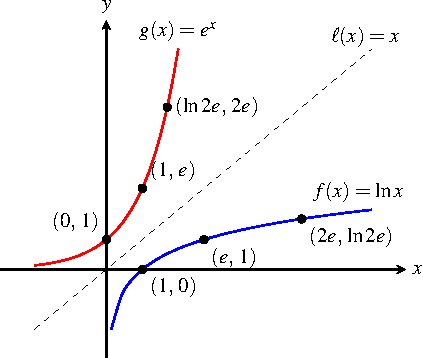
\includegraphics[scale=1.2]{image/12/inverses.pdf}
\caption{%%
  The graph of the natural logarithmic function $f(x) = \ln x$ is
  obtained by reflecting the exponential function $g(x) = e^x$ with
  respect to the line $\ell(x) = x$.
}
\label{fig:logarithmic_function_reflection_of_exponential_function}
\end{figure}

\begin{exercise}
Provide an example of two operations~(different from those presented
above) that are inverses of each other.  Explain how one operation can
be used to undo the result of the other operation.
\end{exercise}

\ifbool{showSolution}{
\begin{solution}
The operations of squaring and square root are inverses of each
other.  Let $x \geq 0$ be any real number.  The square of $x$ is
$x^2$.  To undo the squaring, take the square root of $x^2$ and you
get
\[
\sqrt{x^2}
=
(x^2)^{1/2}
=
x^{2/2}
=
x.
\]
On the other hand, the square root of $x$ is $\sqrt{x}$.  To undo the
square root, you square $\sqrt{x}$ and end up with
\[
\bigparen{\sqrt{x}}^2
=
\bigparen{x^{1/2}}^2
=
x^{2/2}
=
x.
\]
Thus either operation can be used to undo the result of the other
operation.
\end{solution}
}{}

\begin{theorem}
\label{thm:logarithm:cancellation_property}
\textbf{Cancellation property.}
Let $b$ be a positive number such that $b \neq 1$.
%%
\begin{packedenum}
\item\label{subthm:logarithm:cancellation_property_log_exponential}
  If $x$ is any real number, then $\log_b (b^x) = x$.

\item\label{subthm:logarithm:cancellation_property_exponential_log}
  If $x > 0$ is any positive number, then $b^{\log_b x} = x$.
\end{packedenum}
\end{theorem}

\begin{example}
Solve the equation $\log_{10} x = \frac{1}{2}$ for $x$.
\end{example}

\begin{solution}
The equation $\log_{10} x = \frac{1}{2}$ asks you to determine a value
of $x$ such that $\log_{10} x$ evaluates to $1 / 2$.  You can use
\Subtheorem{thm:logarithm:cancellation_property}{subthm:logarithm:cancellation_property_exponential_log}
and consider both sides of $\log_{10} x = \frac{1}{2}$ as exponents of
the base $10$.  Then the latter equation can be written as
\[
10^{\log_{10} x}
=
10^{1/2}
=
\sqrt{10}.
\]
The left-hand side simplifies to $x$ and the equation now becomes
$x = \sqrt{10}$.
\end{solution}

\begin{exercise}
Solve the equation $\log_2 x = 5$ for $x$.
\end{exercise}

\ifbool{showSolution}{
\begin{solution}
You can treat both sides of $\log_2 x = 5$ as exponents of the base
$2$.  Then the latter equation can also be written as
\[
2^{\log_2 x}
=
2^5
\]
which by
\Subtheorem{thm:logarithm:cancellation_property}{subthm:logarithm:cancellation_property_exponential_log}
simplifies to $x = 2^5 = 32$.
\end{solution}
}{}

\begin{exercise}
Solve the equation $\ln 2x = 3$ for $x$.
\end{exercise}

\ifbool{showSolution}{
\begin{solution}
You can treat both sides of the equation $\ln 2x = 3$ as exponents of
the irrational number $e$.  This allows you to write the latter
equation as
\[
e^{\ln 2x}
=
e^3.
\]
Use
\Subtheorem{thm:logarithm:cancellation_property}{subthm:logarithm:cancellation_property_exponential_log}
to simplify the last equation to $2x = e^3$, which upon solving for
$x$ yields $x = \frac{1}{2} e^3$.
\end{solution}
}{}

\begin{exercise}
\textbf{Negative pH.}
In the Richmond Mine at Iron Mountain, California, USA a team of
researchers found that the underground water had a pH value as low as
$-3.6$.\footnote{
  See the paper: \url{https://doi.org/10.1021/es990646v}.
}
Suppose that the water had a pH value of $-3.6$.  Calculate the molar
concentration of hydrogren ions in the water.
\end{exercise}

\ifbool{showSolution}{
\begin{solution}
You have $\text{pH} = -3.6$.  Substitute the latter value into
\Equation{eqn:logarithm:pH} to obtain the equation
\[
-3.6
=
-\log_{10} x
\]
where $x = \molarH$.  The above equation simplifies to
$3.6 = \log_{10} x$, where you can consider both sides as exponents of
$10$.  In other words, you have the equivalent equation
$10^{3.6} = 10^{\log_{10} x}$, which by
\Subtheorem{thm:logarithm:cancellation_property}{subthm:logarithm:cancellation_property_exponential_log}
can be simplified as $10^{3.6} = x$.  Conclude that if the underground
water at Iron Mountain had a pH value of $-3.6$, then the water had a
hydrogen ion concentration of $10^{3.6}$M.
\end{solution}
}{}

\begin{theorem}
\label{thm:logarithm:properties}
\textbf{Properties of logarithm.}
Let $\triple{a}{b}{c}$ be positive numbers such that $b \neq 1$.
%%
\begin{packedenum}
\item\label{thm:logarithm:properties_addition}
  Addition rule:
  $\log_b (ac) = \log_b a + \log_b c$

\item\label{thm:logarithm:properties_subtraction}
  Subtraction rule:
  $\log_b \parenthesis*{\frac{a}{c}} = \log_b a - \log_b c$

\item\label{thm:logarithm:properties_multiplication}
  Power rule:
  If $x$ is any real number, then $\log_b (a^x) = x \cdot \log_b a$.

\item\label{thm:logarithm:properties_log_1}
  Zero rule: $\log_b 1 = 0$

\item\label{thm:logarithm:properties_log_b}
  Unit rule: $\log_b b = 1$
\end{packedenum}
\end{theorem}

\begin{proof}
\solutionpart{thm:logarithm:properties_addition}
Since $\triple{a}{b}{c}$ are positive numbers, there exist numbers $m$
and $n$ such that $a = b^m$ and $c = b^n$.  By
\Subtheorem{thm:logarithm:cancellation_property}{subthm:logarithm:cancellation_property_log_exponential}
you have the identities
%%
\begin{equation}
\label{eqn:logarithm:log_b_a_m_log_b_c_n}
\log_b a = \log_b (b^m) = m
%%
\qquad
\text{and}
\qquad
%%
\log_b c = \log_b (b^n) = n.
\end{equation}
%%
The product of $a$ and $c$ can be written as
$a \cdot c = b^m \cdot b^n$, which simplifies to
$a \cdot c = b^{m + n}$.  In the latter equation, taking the logarithm
to base $b$ of both sides results in
$\log_b (a \cdot c) = \log_b (b^{m+n})$.  Use
\Subtheorem{thm:logarithm:cancellation_property}{subthm:logarithm:cancellation_property_log_exponential}
again to simplify the last equation to $\log_b (a \cdot c) = m+n$,
which by the identities in~\eqref{eqn:logarithm:log_b_a_m_log_b_c_n}
can be written as
$\log_b (a \cdot c) = \log_b a + \log_b c$.

\solutionpart{thm:logarithm:properties_subtraction}
See \Exercise{ex:logarithm:properties_subtraction}.

\solutionpart{thm:logarithm:properties_multiplication}
Since $a$ and $b$ are positive numbers, there exists a number $n$ such
that $a = b^n$.  If $x$ is any real number, raise both sides of the
latter equation to the power of $x$ and you get
$a^x = (b^n)^x$, which simplifies to $a^x = b^{nx}$.  In the last
equation, take the logarithm to base $b$ of both sides and you obtain
$\log_b (a^x) = \log_b (b^{nx})$, which by
\Subtheorem{thm:logarithm:cancellation_property}{subthm:logarithm:cancellation_property_log_exponential}
can also be written as
%%
\begin{equation}
\label{eqn:logarithm:log_b_a_x_nx}
\log_b (a^x)
=
nx.
\end{equation}
%%
In the equation $a = b^n$, taking the logarithm to base $b$ of both
sides produces $\log_b a = \log_b (b^n)$ and using
\Subtheorem{thm:logarithm:cancellation_property}{subthm:logarithm:cancellation_property_log_exponential}
again shows that you can also write $\log_b a = n$.  Substitute the
latter expression into \Equation{eqn:logarithm:log_b_a_x_nx} and you
get $\log_b (a^x) = (\log_b a) \cdot x$, which you can also write as
$\log_b (a^x) = x \cdot \log_b a$.

\solutionpart{thm:logarithm:properties_log_1}
See \Exercise{ex:logarithm:log_b_1_0}.

\solutionpart{thm:logarithm:properties_log_b}
As $b \neq 1$ is positive, use
\Subtheorem{thm:logarithm:cancellation_property}{subthm:logarithm:cancellation_property_exponential_log}
to write $b^{\log_b b} = b$.  Taking the logarithm to base $b$ of both
sides yields $\log_b (b^{\log_b b}) = \log_b b$, which by the power
rule from \Part{thm:logarithm:properties_multiplication} can also be
written as $\log_b b \cdot \log_b b = \log_b b$.  Since $b \neq 1$,
by \Part{thm:logarithm:properties_log_1} you know that
$\log_b b \neq 0$.  Thus in the equation
$\log_b b \cdot \log_b b = \log_b b$ you can divide both sides by
$\log_b b$ to get
\[
\frac{
  \log_b b \cdot \log_b b
}{
  \log_b b
}
=
\frac{\log_b b}{\log_b b}
\]
and simplify the latter expression to $\log_b b = 1$.
\end{proof}

\begin{exercise}
\label{ex:logarithm:properties_subtraction}
Prove
\Subtheorem{thm:logarithm:properties}{thm:logarithm:properties_subtraction}.
\end{exercise}

\ifbool{showSolution}{
\begin{solution}
Since $\triple{a}{b}{c}$ are positive numbers, there exist numbers $m$
and $n$ such that $a = b^m$ and $c = b^n$.  Now use
\Subtheorem{thm:logarithm:cancellation_property}{subthm:logarithm:cancellation_property_log_exponential}
to obtain the identities
%%
\begin{equation}
\label{eqn:logarithm:ex_log_b_a_m_log_b_c_n}
\log_b a = \log_b (b^m) = m
%%
\qquad
\text{and}
\qquad
%%
\log_b c = \log_b (b^n) = n.
\end{equation}
%%
You can write the fraction $a / c$ as
$\frac{a}{c} = \frac{b^m}{b^n}$, which simplifies to
$\frac{a}{c} = b^{m - n}$.  In the latter equation, take the logarithm
to base $b$ of both sides and you end up with
$\log_b \parenthesis*{\frac{a}{c}} = \log_b (b^{m - n})$.  Another
application of
\Subtheorem{thm:logarithm:cancellation_property}{subthm:logarithm:cancellation_property_log_exponential}
shows that the latter equation can be simplified as
$\log_b \parenthesis*{\frac{a}{c}} = m - n$, which by the identities
in~\eqref{eqn:logarithm:ex_log_b_a_m_log_b_c_n} can also be written as
$\log_b \parenthesis*{\frac{a}{c}} = \log_b a - \log_b c$.
\end{solution}
}{}

\begin{exercise}
\label{ex:logarithm:log_b_1_0}
Prove
\Subtheorem{thm:logarithm:properties}{thm:logarithm:properties_log_1}.
\end{exercise}

\ifbool{showSolution}{
\begin{solution}
Let $b > 0$ be any number such that $b \neq 1$.  You know that
$b^0 = 1$.  Take the logarithm to base $b$ of both sides and you
obtain $\log_b (b^0) = \log_b 1$, which by the power rule from
\Subtheorem{thm:logarithm:properties}{thm:logarithm:properties_multiplication}
can also be written as $0 \cdot \log_b b = \log_b 1$.  The latter
equation simplifies to $0 = \log_b 1$.
\end{solution}
}{}

\begin{theorem}
\label{thm:logarithm:change_of_base}
\textbf{Change of base.}
Let $b \neq 1$ and $k \neq 1$ be positive numbers.  If $x > 0$ is any
number, then
\[
\log_b x
=
\frac{
  \log_k x
}{
  \log_k b
}.
\]
\end{theorem}

\begin{proof}
Use
\Subtheorem{thm:logarithm:cancellation_property}{subthm:logarithm:cancellation_property_exponential_log}
to write $b^{\log_b x} = x$.  Take the logarithm to base $k$ of both
sides and you end up with
$\log_k \parenthesis*{b^{\log_b x}} = \log_k x$, which
by
\Subtheorem{thm:logarithm:properties}{thm:logarithm:properties_multiplication}
can also be written as
\[
\log_b x \cdot \log_k b
=
\log_k x.
\]
Solve the latter equation for $\log_b x$ to get the result.
\end{proof}

\Theorem{thm:logarithm:change_of_base} is most useful in cases where
an electronic calculator or computer program cannot directly evaluate
the logarithm of a number to any positive base you want.  The reason
might be that the calculator~(respectively, program) does not have a
buttom or command to evaluate the logarithm to an arbitrary base.
Consider again
\Equation{eqn:logarithm:Australia_population_doubling_time}, which is
repeated below for reference:
\[
\log_{1.016} \frac{30}{24.7029}
=
t.
\]
Here, the base of the logarithm is $b = 1.016$.  Use
\Subtheorem{thm:logarithm:properties}{thm:logarithm:properties_subtraction}
to write the latter equation as
%%
\begin{equation}
\label{eqn:logarithm:Australia_population_doubling_time_change_of_base}
\begin{aligned}
\log_{1.016} \frac{30}{24.7029}
&=
\log_{1.016} 30 - \log_{1.016} 24.7029 \\[4pt]
&=
t.
\end{aligned}
\end{equation}
%%
If your calculator or computer program does not have a buttom or
command for the logarithm to base $1.016$, use
\Theorem{thm:logarithm:change_of_base} to change the base to a more
convenient base such as base $e$.  With the base of $e$, you can now
write
\[
\log_{1.016} 30
=
\frac{
  \ln 30
}{
  \ln 1.016
}
%%
\qquad
\text{and}
\qquad
%%
\log_{1.016} 24.7029
=
\frac{
  \ln 24.7029
}{
  \ln 1.016
}
\]
which can be used to write
\Expression{eqn:logarithm:Australia_population_doubling_time_change_of_base}
as
%%
\begin{align*}
t
&=
\frac{
  \ln 30
}{
  \ln 1.016
}
-
\frac{
  \ln 24.7029
}{
  \ln 1.016
} \\[4pt]
&=
\frac{
  \ln 30 - \ln 24.7029
}{
  \ln 1.016
}.
\end{align*}
%%
The latter expression can be evaluated by any calculator or computer
program that implements the natural logarithm.

\begin{exercise}
Consider the expression $\log_2 256$.  Without using a calculator or
computer program:
%%
\begin{packedenum}
\item\label{subex:logarithm:log_2_256_properties}
  Simplify the expression by means of the properties of logarithm.

\item\label{subex:logarithm:log_2_256_change_base}
  Simplify the expression by first changing the base from $2$ to $e$.
\end{packedenum}
\end{exercise}

\ifbool{showSolution}{
\begin{solution}
\solutionpart{subex:logarithm:log_2_256_properties}
Note that $256 = 2^8$.  You can write $\log_2 256 = \log_2 (2^8)$.
Use the power rule of
\Subtheorem{thm:logarithm:properties}{thm:logarithm:properties_multiplication}
to write $\log_2 (2^8) = 8 \cdot \log_2 2$, which by the unit rule of
\Subtheorem{thm:logarithm:properties}{thm:logarithm:properties_log_b}
simplifies to $\log_2 (2^8) = 8 \cdot 1 = 8$.  Therefore $\log_2 256$
evaluates to $\log_2 256 = 8$.

\solutionpart{subex:logarithm:log_2_256_change_base}
By using \Theorem{thm:logarithm:change_of_base}, you change the base
of $\log_2 256$ to base $e$ as follows:
\[
\log_2 256
=
\frac{
  \ln 256
}{
  \ln 2
}.
\]
Since $\ln 256 = \ln (2^8)$, use the power rule of
\Subtheorem{thm:logarithm:properties}{thm:logarithm:properties_multiplication}
to write
\[
\log_2 256
=
\frac{
  \ln (2^8)
}{
  \ln 2
}
=
\frac{
  8 \cdot \ln 2
}{
  \ln 2
}.
\]
The right-hand side simplifies to $8$, hence $\log_2 256 = 8$.
\end{solution}
}{}

\begin{exercise}
\textbf{Newton's law of cooling.}
Let $T_0$ be the original temperature of an object and suppose that
$T_s$ represent the constant temperature of the environment
surrounding the object, all temperatures measured in degrees Celsius.
If $T(t)$ represents the temperature of an object after $t$ units of
time, Newton's law of cooling states that $T(t)$ can be written as
%%
\begin{equation}
\label{eqn:logarithm:Newton_law_cooling}
T(t)
=
T_s + (T_0 - T_s) e^{-kt}
\end{equation}
%%
where $k > 0$ is the rate of cooling written as a decimal.  Here, it
is assumed that the surrounding maintains a constant temperature.
Suppose a pot of soup has a tempature of $\degreec{100}$ and that the
temperature of the surrounding is $\degreec{15}$.  You place the pot
of soup on the kitchen bench and let the soup cool.  After one hour, the
temperature of the soup drops down to $\degreec{50}$.
%%
\begin{packedenum}
\item\label{subex:logarithm:Newton_law_cooling_soup_formula}
  Assume that the surrounding maintains a constant temperature of
  $\degreec{15}$.  Derive a formula for the temperature $T(t)$ of the
  soup after $t$ hours.

\item\label{subex:logarithm:Newton_law_cooling_soup_20}
  If the surrounding continues to maintain a constant temperature of
  $\degreec{15}$, how long must you wait for the temperature of the
  soup to be $\degreec{20}$?
\end{packedenum}
\end{exercise}

\ifbool{showSolution}{
\begin{solution}
\solutionpart{subex:logarithm:Newton_law_cooling_soup_formula}
First, you must determine the rate $k$ of cooling.  The original
temperature of the pot of soup is $T_0 = 100$ degrees Celsius.  The
surrounding maintains a constant temperature of $T_s = 15$ degrees
Celsius.  After one hour, the temperature of the soup decreases to
$\degreec{50}$, which you can write as the expression $T(1) = 50$.
Substitute the known values into
\Equation{eqn:logarithm:Newton_law_cooling} and you end up with
%%
\begin{align*}
50
&=
15 + (100 - 15) e^{-k \times 1} \\[4pt]
&=
15 + 85 e^{-k}.
\end{align*}
%%
You need to solve the latter equation for $k$.  The last equation can
also be written as $50 - 15 = 85 e^{-k}$.  Divide both sides by $85$
and you get $\frac{50 - 15}{85} = e^{-k}$, which simplifies to
$\frac{7}{17} = e^{-k}$.  In the last equation, take the natural
logarithm of both sides and you have
$\ln \parenthesis*{\frac{7}{17}} = \ln (e^{-k})$, which by
\Subtheorem{thm:logarithm:cancellation_property}{subthm:logarithm:cancellation_property_log_exponential}
can be simplified as $\ln \parenthesis*{\frac{7}{17}} = -k$.  Solve
the last equation for $k$ and you get
%%
\begin{equation}
\label{eqn:logarithm:Newton_law_cooling_rate_k}
\begin{aligned}
k
&=
-\ln \parenthesis*{\frac{7}{17}} \\[4pt]
&=
-(\ln 7 - \ln 17) \\[4pt]
&=
\ln 17 - \ln 7 \\[4pt]
&=
\ln \parenthesis*{\frac{17}{7}}.
\end{aligned}
\end{equation}
%%
You now have all information necessary to substitute into
\Equation{eqn:logarithm:Newton_law_cooling}.  Substitution and
simplifying yield the formula
\[
T(t)
=
15 + 85 e^{-kt}
\]
where $k$ is defined as per
\Expression{eqn:logarithm:Newton_law_cooling_rate_k}.

\solutionpart{subex:logarithm:Newton_law_cooling_soup_20}
You want a value of $t$ such that $T(t) = 20$ degrees Celsius.  That
is, you want to solve the equation $20 = 15 + 85 e^{-kt}$ for $t$,
where $k$ is defined as in
\Expression{eqn:logarithm:Newton_law_cooling_rate_k}.  The latter
equation can be written as $20 - 15 = 85 e^{-kt}$ or
$\frac{20 - 15}{85} = e^{-kt}$, which simplifies to
$\frac{1}{17} = e^{-kt}$.  Take the natural logarithm of both sides
and you have $\ln \parenthesis*{\frac{1}{17}} = \ln (e^{-kt})$, which
by
\Subtheorem{thm:logarithm:cancellation_property}{subthm:logarithm:cancellation_property_log_exponential}
simplifies to $\ln \parenthesis*{\frac{1}{17}} = -kt$.  Solving the
last equation for $t$ produces the expression
%%
\begin{align*}
t
&=
-\frac{1}{k} \ln \parenthesis*{\frac{1}{17}} \\[4pt]
&\approx
3.1931
\end{align*}
%%
rounded to four decimal places.  Therefore you must wait approximately
$3.1931$ hours for the soup to cool down to $\degreec{20}$.
\end{solution}
}{}


%%%%%%%%%%%%%%%%%%%%%%%%%%%%%%%%%%%%%%%%%%%%%%%%%%%%%%%%%%%%%%%%%%%%%%%%%%%

\section{Logarithmic plots}

Another useful property of logarithm is that it can scale down large
numbers and scale up small numbers.  This is especially useful if your
data set consists of, for example, numbers that range from the
hundreds to the billions.  In that case, you should consider plotting
your data set with a logarithmic axis.


%%%%%%%%%%%%%%%%%%%%%%%%%%%%%%%%%%%%%%%%%%%%%%%%%%%%%%%%%%%%%%%%%%%%%%%%%%%

\subsection{Logarithmic on vertical axis}

By way of an example, consider the graphs in
\Figure{fig:logarithm:rainbow_trout}.  Each graph shows the same data
set on the total length versus weight of $42$ rainbow trout; see
\Table{tab:logarithm:rainbow_trout}.\footnote{
  The data set was published in the following document:
  \url{http://web.archive.org/web/20180513070421/https://fortress.wa.gov/ecy/publications/documents/0003017.pdf},
  accessed 2018-05-13.
}
\Figure{fig:logarithm:rainbow_trout_linear} shows the scatter plot
with the usual linear scale for the horizontal and vertical axes.  Up
to now, you have been producing scatter plots with linear scaling.
Note that \Figure{fig:logarithm:rainbow_trout_log} shows the same
scatter plot, but each value on the vertical axis has been transformed
to its equivalent under the common logarithm.  The graph in
\Figure{fig:logarithm:rainbow_trout_log} is called a \emph{semi-log}
plot because the common logarithm was taken of each value on only one
axis, in particular the vertical axis.

\begin{figure}[!htbp]
\centering
\subfigure[]{
  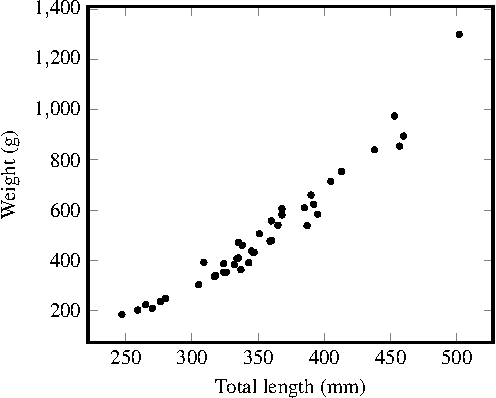
\includegraphics[scale=0.79]{image/12/rainbow-trout-linear.pdf}
  \label{fig:logarithm:rainbow_trout_linear}
}
%%
%%
\subfigure[]{
  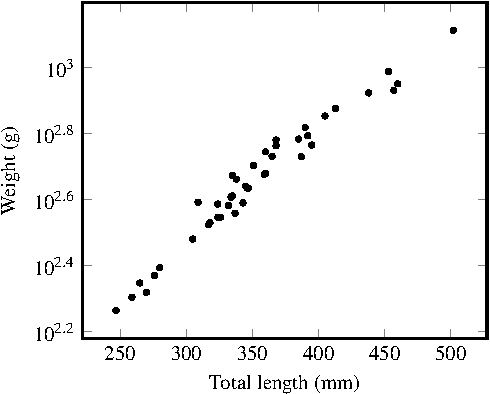
\includegraphics[scale=0.79]{image/12/rainbow-trout-log.pdf}
  \label{fig:logarithm:rainbow_trout_log}
}
\caption{%%
  The total length versus weight of $42$ rainbow trout.  The trout
  were sampled from four different locations along the Spokane River,
  Washington, USA during the months of July, August, and October of
  1999.  The total length of each trout was measured in millimetres
  and the weight was measured in grams.  (a)~A scatter plot with
  linear axes.  (b)~A scatter plot with semi-log axes.
}
\label{fig:logarithm:rainbow_trout}
\end{figure}

As you can see from \Figure{fig:logarithm:rainbow_trout_log}, a
semi-log plot can be used to linearise a data set.  If a data set
approximately follows an exponential model $Q(x)$, a semi-log plot
should allow you to visualise the data set as points around a straight
line.  In other words, if the semi-log plot shows that the points seem
to lie around a straight line, then you should try to model the
original data set via an exponential function.  To do so, first you
must linearise the data by taking the (usually natural) logarithm of
the $y$ column.  Second, you use linear regression to determine a
linear function $f(x)$ that best fits the linearised data.  Finally,
you transform $f(x)$ into the exponential function $Q(x)$.  In
particular, suppose that the data set approximately follows the
exponential function
%%
\begin{equation}
\label{eqn:logarithm:exponential_model}
Q(x)
=
a \cdot e^{rx}.
\end{equation}
%%
The values of the parameters $a$ and $r$ can be estimated as follows.
Take the natural logarithm of both sides of
\Equation{eqn:logarithm:exponential_model} and you get
$\ln Q(x) = \ln (a \cdot e^{rx})$.  Use the addition rule of
\Subtheorem{thm:logarithm:properties}{thm:logarithm:properties_addition}
to write the latter equation as $\ln Q(x) = \ln a + \ln (e^{rx})$,
which by
\Subtheorem{thm:logarithm:cancellation_property}{subthm:logarithm:cancellation_property_log_exponential}
simplifies to
%%
\begin{equation}
\label{eqn:logarithm:exponential_linearised}
\ln Q(x)
=
rx + \ln a.
\end{equation}
%%
Note that~\eqref{eqn:logarithm:exponential_linearised} is a linear
equation, where the vertical intercept and rate of change are $\ln a$
and $r$, respectively.  Use linear regression to estimate $r$ as
$\alphahat$ and $\ln a$ as $\betahat$.  Now $\alphahat$ is an estimate
of $r$ in \Equation{eqn:logarithm:exponential_model} and
$e^{\betahat}$ is an estimate of $a$
in~\eqref{eqn:logarithm:exponential_model}.
\Example{ex:logarithm:rainbow_trout} below clarifies the above
technique for estimating the parameters of an exponential model.

\begin{table}[!htbp]
\centering
\begin{tabular}{cccrrrr} \toprule
$x$   & $w$    & $y$      & $d(x_i)$    & $d(y_i)$  & $d(x_i) d(y_i)$ & $d(x_i) d(x_i)$ \\\midrule
$457$ & $855$  & $6.7511$ & $104.1429$  & $0.6301$  & $65.6217$      & $10845.7347$    \\
$405$ & $715$  & $6.5723$ & $52.1429$   & $0.4513$  & $23.5317$      & $2718.8776$     \\
$453$ & $975$  & $6.8824$ & $100.1429$  & $0.7614$  & $76.2536$      & $10028.5918$    \\
$460$ & $895$  & $6.7968$ & $107.1429$  & $0.6758$  & $72.4109$      & $11479.5918$    \\
$335$ & $472$  & $6.1570$ & $-17.8571$  & $0.0360$  & $-0.6427$      & $318.8776$      \\
$365$ & $540$  & $6.2916$ & $12.1429$   & $0.1706$  & $2.0713$       & $147.4490$      \\
$390$ & $660$  & $6.4922$ & $37.1429$   & $0.3713$  & $13.7893$      & $1379.5918$     \\
$368$ & $581$  & $6.3648$ & $15.1429$   & $0.2438$  & $3.6913$       & $229.3061$      \\
$385$ & $609$  & $6.4118$ & $32.1429$   & $0.2908$  & $9.3481$       & $1033.1633$     \\
$360$ & $557$  & $6.3226$ & $7.1429$    & $0.2016$  & $1.4398$       & $51.0204$       \\
$346$ & $433$  & $6.0707$ & $-6.8571$   & $-0.0503$ & $0.3446$       & $47.0204$       \\
$438$ & $840$  & $6.7334$ & $85.1429$   & $0.6124$  & $52.1426$      & $7249.3061$     \\
$392$ & $623$  & $6.4345$ & $39.1429$   & $0.3136$  & $12.2735$      & $1532.1633$     \\
$324$ & $387$  & $5.9584$ & $-28.8571$  & $-0.1626$ & $4.6911$       & $832.7347$      \\
$360$ & $479$  & $6.1717$ & $7.1429$    & $0.0507$  & $0.3622$       & $51.0204$       \\
$413$ & $754$  & $6.6254$ & $60.1429$   & $0.5044$  & $30.3363$      & $3617.1633$     \\
$276$ & $235$  & $5.4596$ & $-76.8571$  & $-0.6614$ & $50.8336$      & $5907.0204$     \\
$387$ & $538$  & $6.2879$ & $34.1429$   & $0.1669$  & $5.6974$       & $1165.7347$     \\
$345$ & $438$  & $6.0822$ & $-7.8571$   & $-0.0388$ & $0.3046$       & $61.7347$       \\
$395$ & $584$  & $6.3699$ & $42.1429$   & $0.2489$  & $10.4899$      & $1776.0204$     \\
$326$ & $353$  & $5.8665$ & $-26.8571$  & $-0.2545$ & $6.8357$       & $721.3061$      \\
$270$ & $209$  & $5.3423$ & $-82.8571$  & $-0.7787$ & $64.5171$      & $6865.3061$     \\
$359$ & $476$  & $6.1654$ & $6.1429$    & $0.0444$  & $0.2729$       & $37.7347$       \\
$347$ & $432$  & $6.0684$ & $-5.8571$   & $-0.0526$ & $0.3079$       & $34.3061$       \\
$259$ & $202$  & $5.3083$ & $-93.8571$  & $-0.8127$ & $76.2797$      & $8809.1633$     \\
$247$ & $184$  & $5.2149$ & $-105.8571$ & $-0.9061$ & $95.9122$      & $11205.7347$    \\
$280$ & $248$  & $5.5134$ & $-72.8571$  & $-0.6076$ & $44.2651$      & $5308.1633$     \\
$265$ & $223$  & $5.4072$ & $-87.8571$  & $-0.7138$ & $62.7139$      & $7718.8776$     \\
$309$ & $392$  & $5.9713$ & $-43.8571$  & $-0.1497$ & $6.5666$       & $1923.4490$     \\
$338$ & $460$  & $6.1312$ & $-14.8571$  & $0.0102$  & $-0.1521$      & $220.7347$      \\
$334$ & $406$  & $6.0064$ & $-18.8571$  & $-0.1146$ & $2.1617$       & $355.5918$      \\
$332$ & $383$  & $5.9480$ & $-20.8571$  & $-0.1730$ & $3.6073$       & $435.0204$      \\
$324$ & $353$  & $5.8665$ & $-28.8571$  & $-0.2545$ & $7.3447$       & $832.7347$      \\
$337$ & $363$  & $5.8944$ & $-15.8571$  & $-0.2266$ & $3.5930$       & $251.4490$      \\
$343$ & $390$  & $5.9661$ & $-9.8571$   & $-0.1548$ & $1.5263$       & $97.1633$       \\
$318$ & $340$  & $5.8289$ & $-34.8571$  & $-0.2920$ & $10.1798$      & $1215.0204$     \\
$305$ & $303$  & $5.7137$ & $-47.8571$  & $-0.4073$ & $19.4901$      & $2290.3061$     \\
$335$ & $410$  & $6.0162$ & $-17.8571$  & $-0.1048$ & $1.8720$       & $318.8776$      \\
$317$ & $335$  & $5.8141$ & $-35.8571$  & $-0.3069$ & $11.0031$      & $1285.7347$     \\
$351$ & $506$  & $6.2265$ & $-1.8571$   & $0.1055$  & $-0.1960$      & $3.4490$        \\
$368$ & $605$  & $6.4052$ & $15.1429$   & $0.2842$  & $4.3042$       & $229.3061$      \\
$502$ & $1300$ & $7.1701$ & $149.1429$  & $1.0491$  & $156.4704$     & $22243.5918$    \\\bottomrule
\end{tabular}

\caption{%%
  The total length $x$ versus weight $w$ of $42$ rainbow trout.  Total
  length is measured in millimetres and weight is measured in grams.
  Each $y_i$ is the natural logarithm of $w_i$.  If $\xbar$ and
  $\ybar$ are the means of the $x$ and $y$ columns, respectively, then
  $d(x_i) = x_i - \xbar$ and $d(y_i) = y_i - \ybar$.  The whole table
  shows the detailed calculation necessary for the linear regression
  of the $x$ and $y$ columns.
}
\label{tab:logarithm:rainbow_trout}
\end{table}

\begin{example}
\label{ex:logarithm:rainbow_trout}
\textbf{Rainbow trout.}
Suppose that the rainbow trout data set shown in
\Figure{fig:logarithm:rainbow_trout} follows the exponential
model~\eqref{eqn:logarithm:exponential_model}.
%%
\begin{packedenum}
\item\label{subex:logarithm:trout_logarithm}
  Take the natural logarithm of each weight value.

\item\label{subex:logarithm:trout_linear_regression}
  Use linear regression to estimate the parameters $a$ and $r$.

\item\label{subex:logarithm:trout_formula_graph}
  Use your estimates
  from \Part{subex:logarithm:trout_linear_regression} to write a
  formula for the weight $Q(x)$~(in grams) of a rainbow trout that has
  a total length of $x$ millimetres.  Graph your formula together with
  the data in the $x$ and $w$ columns of
  \Table{tab:logarithm:rainbow_trout}.
\end{packedenum}
\end{example}

\begin{solution}
\solutionpart{subex:logarithm:trout_logarithm}
In \Table{tab:logarithm:rainbow_trout}, the $x$ and $w$ columns show
the total length~(mm) and corresponding weight~(g) of $42$ rainbow
trout.  \Figure{fig:logarithm:rainbow_trout_linear} is a scatter plot
of the $x$ column versus the $w$ column.  If you transform each weight
value to its equivalent under the natural logarithm, the result is
shown in the $y$ column.  That is, if $w_i$ is the weight of trout
$i$, then $y_i = \ln w_i$.  \Figure{fig:logarithm:rainbow_trout_log}
is a scatter plot of the $x$ column versus the $y$ column.

\solutionpart{subex:logarithm:trout_linear_regression}
The linear regression function has the form
\[
y
=
\ln w
=
rx + \ln a
\]
where you want to estimate the parameters $r$ and $\ln a$.  Note that
$y$ is the natural logarithm of the weight $w$.  If $\alphahat$ and
$\betahat$ are estimates of $r$ and $\ln a$, respectively, then the
estimates can be written as
%%
\begin{equation}
\label{eqn:logarithm:linear_regression_alpha_hat_beta_hat}
\begin{aligned}
\alphahat
&=
\frac{
  \sum_{i=1}^n (x_i - \xbar) (y_i - \ybar)
}{
  \sum_{i=1}^n (x_i - \xbar)^2
} \\[4pt]
%%
%%
\betahat
&=
\ybar - \alphahat \xbar
\end{aligned}
\end{equation}
%%
where $n$ is the number of data points.  In this example, you have
$n = 42$ data points for $42$ rainbow trout.  The means of the $x$ and
$y$ columns are $\xbar \approx 352.8571$ and
$\ybar \approx 6.1210$, respectively, each number rounded to four
decimal places.  \Table{tab:logarithm:rainbow_trout} shows the
detailed calculations of the numbers $d(x_i) = x_i - \xbar$ and
$d(y_i) = y_i - \ybar$ and the products $d(x_i) d(y_i)$ and
$d(x_i) d(x_i)$.  Numbers in the table have been rounded to four
decimal places in order to fit the table.  However, when you do your
own calculations you should use a spreadsheet software package and not
round any intermediate results.  Using the numbers in the table, you
have the sums
\[
\sum_{i=1}^n (x_i - \xbar) (y_i - \ybar)
\approx
1013.8665
%%
\qquad
\text{and}
\qquad
%%
\sum_{i=1}^n (x_i - \xbar)^2
\approx
132875.1429
\]
both numbers rounded to four decimal places.  Now use the equations
in~\eqref{eqn:logarithm:linear_regression_alpha_hat_beta_hat} to
estimate $\alphahat$ and $\betahat$ as
\[
\alphahat
\approx
0.0076
%%
\qquad
\text{and}
\qquad
%%
\betahat
\approx
3.4286
\]
rounded to four decimal places.  Note that $\alphahat$ is an estimate
of $r$ in the model $Q(x) = a \cdot e^{rt}$ and $\betahat$ is an
estimate of $\ln a$.  Then you have the equation $\betahat = \ln a$.
Treat both sides of the last equation as exponents of $e$ and you end
up with $e^{\betahat} = e^{\ln a}$, which simplifies to
$e^{\betahat} = a$.  Thus the parameter $r$ can be estimated as
$r \approx 0.0076$ and $a$ can be estimated as $a \approx 30.8338$.

\begin{figure}[!htbp]
\centering
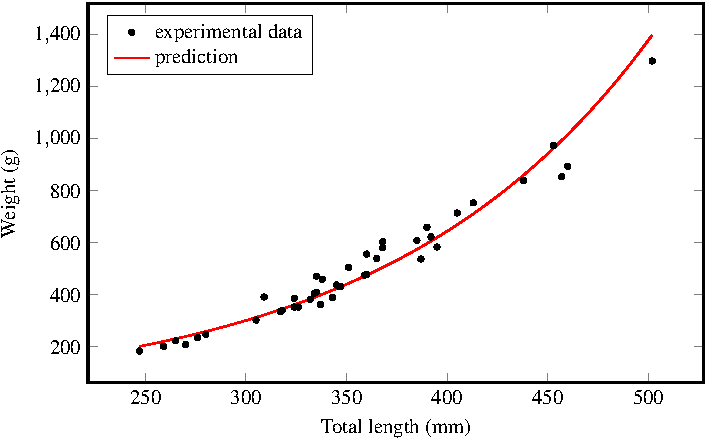
\includegraphics[scale=1.1]{image/12/rainbow-trout.pdf}
\caption{%%
  The total length versus weight of $42$ rainbow trout.  The
  experimental data are from \Table{tab:logarithm:rainbow_trout}.  The
  red curve is a graph of
  \Equation{eqn:logarithm:rainbow_trout_prediction}.
}
\label{fig:rainbow_trout_prediction}
\end{figure}

\solutionpart{subex:logarithm:trout_formula_graph}
Using the estimates
from \Part{subex:logarithm:trout_linear_regression}, if $Q(x)$
represents the weight~(g) of a rainbow trout that has a total length
of $x$~(mm), then $Q(x)$ can be written as
%%
\begin{equation}
\label{eqn:logarithm:rainbow_trout_prediction}
Q(x)
=
30.8338 \cdot e^{0.0076 x}.
\end{equation}
%%
\Figure{fig:rainbow_trout_prediction} shows a graph of
\Equation{eqn:logarithm:rainbow_trout_prediction} together with the
experimental data.
\end{solution}

\begin{exercise}
In \Example{ex:logarithm:rainbow_trout}, calculate the root mean
square error of
\Equation{eqn:logarithm:rainbow_trout_prediction} and the correlation
coefficient of the model.
\end{exercise}

\ifbool{showSolution}{
\begin{solution}
The root mean square error of
\Equation{eqn:logarithm:rainbow_trout_prediction} is $50.1968$,
rounded to four decimal places.  The model has a correlation
coefficient of $0.9792$, rounded to four decimal places.
\end{solution}
}{}

\begin{table}[!htbp]
\centering
\begin{tabular}{ccrrcc} \toprule
Time  & Count && Time   & Count \\\midrule
$0$   & $787$ && $603$  & $236$ \\
$30$  & $738$ && $633$  & $179$ \\
$60$  & $667$ && $663$  & $212$ \\
$90$  & $654$ && $693$  & $189$ \\
$121$ & $565$ && $723$  & $170$ \\
$151$ & $527$ && $753$  & $178$ \\
$181$ & $556$ && $784$  & $160$ \\
$211$ & $505$ && $814$  & $124$ \\
$241$ & $474$ && $844$  & $140$ \\
$271$ & $407$ && $874$  & $114$ \\
$302$ & $368$ && $904$  & $131$ \\
$332$ & $393$ && $934$  & $117$ \\
$362$ & $334$ && $964$  & $140$ \\
$392$ & $327$ && $995$  & $94$  \\
$422$ & $312$ && $1025$ & $107$ \\
$452$ & $293$ && $1055$ & $103$ \\
$482$ & $278$ && $1085$ & $94$  \\
$512$ & $249$ && $1115$ & $79$  \\
$543$ & $250$ && $1145$ & $94$  \\
$573$ & $238$ && $1175$ & $68$  \\\bottomrule
\end{tabular}

\caption{%%
  The radioactive decay of a sample of $9.7656$ grams of copper.  The
  sample was neutron activated for $66$ minutes.  Then a Geiger
  counter was used to measure the number of radioactive isotopes after
  the elapse of the listed number of seconds.  The experiment was
  performed by Steven Sahyun at the University of Wisconsin at
  Whitewater, USA on $13$-th January~$2005$.
}
\label{tab:logarithm:copper_radioactive_decay}
\end{table}

\begin{exercise}
\textbf{Radioactive decay of copper.}
\Table{tab:logarithm:copper_radioactive_decay} shows the radioactive
decay of a sample of copper.\footnote{
  The data set was available at:
  \url{http://web.archive.org/web/20180515171532/http://sahyun.net/physics/neutron/data/Cu_data_2.xls},
  accessed 2018-05-16.
}
The columns for ``Time'' list the elapsed time in seconds, while the
columns for ``Count'' list the corresponding number of radioactive
isotopes as measured by a Geiger counter.
%%
\begin{packedenum}
\item\label{subex:logarithm:copper_decay_linear_log_plots}
  Plot the data in the table by using a linear scale for both the
  horizontal and vertical axes.  What do you notice in the linear
  plot?  Now take the natural logarithm of each value in the ``Count''
  columns and produce a semi-log plot.  What do you notice in the
  semi-log plot?

\item\label{subex:logarithm:copper_decay_regression}
  Suppose that the data in
  \Table{tab:logarithm:copper_radioactive_decay} follow the
  exponential model $Q(x) = a \cdot e^{rx}$, whose logarithmic
  transformation is $\ln Q(x) = rx + \ln a$.  Use linear regression to
  estimate the parameters $r$ and $\ln a$.  Use the estimate for
  $\ln a$ to calculate an estimation of $a$.  Graph the model $Q(x)$
  together with the linear plot
  from \Part{subex:logarithm:copper_decay_linear_log_plots}.

\item\label{subex:logarithm:copper_decay_RMS_error_Pearson_rho}
  Calculate the root mean square~(RMS) error of your model $Q(x)$
  from \Part{subex:logarithm:copper_decay_regression}.  Determine the
  Pearson correlation coefficient $\rho$ of the model.  Provide an
  interpretation of the values of $\rho$ and the RMS error.
\end{packedenum}
\end{exercise}

\ifbool{showSolution}{
\begin{solution}
\solutionpart{subex:logarithm:copper_decay_linear_log_plots}
\Figure{subfig:logarithm:copper_decay_linear} shows a scatter plot of
the data in \Table{tab:logarithm:copper_radioactive_decay}, where the
horizontal and vertical axes use linear scaling.  The graph suggests
that the points roughly follow a model of exponential decay.
\Figure{subfig:logarithm:copper_decay_log} shows a semi-log plot of
the same data set, but with logarithmic scaling for the vertical
axis.  The graph shows that the points seem to lie around a straight
whose gradient is negative.  This further demonstrates that the data
set might be modelled as a function for exponential decay.

\begin{figure}[!htbp]
\centering
\subfigure[]{
  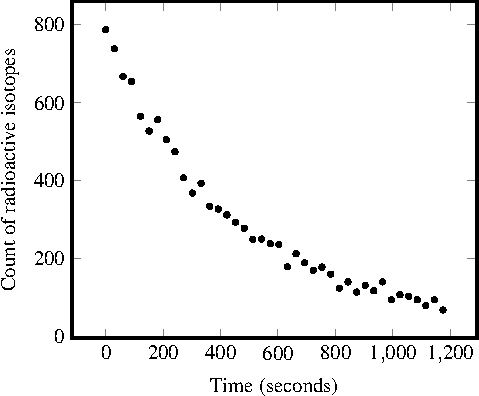
\includegraphics[scale=0.81]{image/12/copper-decay-linear.pdf}
  \label{subfig:logarithm:copper_decay_linear}
}
%%
%%
\subfigure[]{
  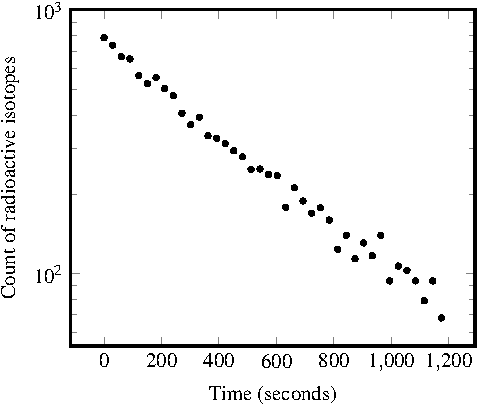
\includegraphics[scale=0.81]{image/12/copper-decay-log.pdf}
  \label{subfig:logarithm:copper_decay_log}
}
\caption{%%
  The radioactive decay of a sample of copper that had been neutron
  activated.  Data are from
  \Table{tab:logarithm:copper_radioactive_decay}.  (a)~A scatter plot
  of the time in seconds versus the count of radioactive isotopes with
  linear axes.  (b)~A semi-log plot of the same data set, where the
  vertical axis uses logarithmic scaling.
}
\label{fig:logarithm:copper_decay}
\end{figure}

\begin{table}[!htbp]
\centering
\begin{tabular}{rrrrrr} \toprule
$x$    & $y$      & $d(x_i)$   & $d(y_i)$  & $d(x_i)d(y_i)$ & $d(x_i)d(x_i)$ \\\midrule
$0$    & $6.6682$ & $-587.725$ & $1.2215$  & $-717.9189$   & $345420.6756$  \\
$30$   & $6.6039$ & $-557.725$ & $1.1572$  & $-645.4202$   & $311057.1756$  \\
$60$   & $6.5028$ & $-527.725$ & $1.0561$  & $-557.3217$   & $278493.6756$  \\
$90$   & $6.4831$ & $-497.725$ & $1.0364$  & $-515.8426$   & $247730.1756$  \\
$121$  & $6.3368$ & $-466.725$ & $0.8901$  & $-415.4409$   & $217832.2256$  \\
$151$  & $6.2672$ & $-436.725$ & $0.8205$  & $-358.3303$   & $190728.7256$  \\
$181$  & $6.3208$ & $-406.725$ & $0.8741$  & $-355.5028$   & $165425.2256$  \\
$211$  & $6.2246$ & $-376.725$ & $0.7779$  & $-293.0363$   & $141921.7256$  \\
$241$  & $6.1612$ & $-346.725$ & $0.7145$  & $-247.7353$   & $120218.2256$  \\
$271$  & $6.0088$ & $-316.725$ & $0.5621$  & $-178.0333$   & $100314.7256$  \\
$302$  & $5.9081$ & $-285.725$ & $0.4614$  & $-131.8268$   & $81638.7756$   \\
$332$  & $5.9738$ & $-255.725$ & $0.5271$  & $-134.7935$   & $65395.2756$   \\
$362$  & $5.8111$ & $-225.725$ & $0.3644$  & $-82.2620$    & $50951.7756$   \\
$392$  & $5.7900$ & $-195.725$ & $0.3433$  & $-67.1833$    & $38308.2756$   \\
$422$  & $5.7430$ & $-165.725$ & $0.2963$  & $-49.1038$    & $27464.7756$   \\
$452$  & $5.6802$ & $-135.725$ & $0.2335$  & $-31.6872$    & $18421.2756$   \\
$482$  & $5.6276$ & $-105.725$ & $0.1809$  & $-19.1272$    & $11177.7756$   \\
$512$  & $5.5175$ & $-75.725$  & $0.0707$  & $-5.3573$     & $5734.2756$    \\
$543$  & $5.5215$ & $-44.725$  & $0.0748$  & $-3.3434$     & $2000.3256$    \\
$573$  & $5.4723$ & $-14.725$  & $0.0256$  & $-0.3764$     & $216.8256$     \\
$603$  & $5.4638$ & $15.275$   & $0.0171$  & $0.2616$      & $233.3256$     \\
$633$  & $5.1874$ & $45.275$   & $-0.2593$ & $-11.7407$    & $2049.8256$    \\
$663$  & $5.3566$ & $75.275$   & $-0.0901$ & $-6.7838$     & $5666.3256$    \\
$693$  & $5.2417$ & $105.275$  & $-0.2050$ & $-21.5771$    & $11082.8256$   \\
$723$  & $5.1358$ & $135.275$  & $-0.3109$ & $-42.0581$    & $18299.3256$   \\
$753$  & $5.1818$ & $165.275$  & $-0.2649$ & $-43.7851$    & $27315.8256$   \\
$784$  & $5.0752$ & $196.275$  & $-0.3715$ & $-72.9226$    & $38523.8756$   \\
$814$  & $4.8203$ & $226.275$  & $-0.6264$ & $-141.7443$   & $51200.3756$   \\
$844$  & $4.9416$ & $256.275$  & $-0.5051$ & $-129.4353$   & $65676.8756$   \\
$874$  & $4.7362$ & $286.275$  & $-0.7105$ & $-203.4007$   & $81953.3756$   \\
$904$  & $4.8752$ & $316.275$  & $-0.5715$ & $-180.7541$   & $100029.8756$  \\
$934$  & $4.7622$ & $346.275$  & $-0.6845$ & $-237.0365$   & $119906.3756$  \\
$964$  & $4.9416$ & $376.275$  & $-0.5051$ & $-190.0430$   & $141582.8756$  \\
$995$  & $4.5433$ & $407.275$  & $-0.9034$ & $-367.9370$   & $165872.9256$  \\
$1025$ & $4.6728$ & $437.275$  & $-0.7739$ & $-338.3973$   & $191209.4256$  \\
$1055$ & $4.6347$ & $467.275$  & $-0.8120$ & $-379.4168$   & $218345.9256$  \\
$1085$ & $4.5433$ & $497.275$  & $-0.9034$ & $-449.2440$   & $247282.4256$  \\
$1115$ & $4.3694$ & $527.275$  & $-1.0773$ & $-568.0115$   & $278018.9256$  \\
$1145$ & $4.5433$ & $557.275$  & $-0.9034$ & $-503.4487$   & $310555.4256$  \\
$1175$ & $4.2195$ & $587.275$  & $-1.2272$ & $-720.7032$   & $344891.9256$  \\\bottomrule
\end{tabular}

\caption{%%
  Detailed calulation of the regression of the data in
  \Table{tab:logarithm:copper_radioactive_decay}.  The column with the
  heading $x$ lists the elapsed times in seconds.  The column with the
  heading $y$ lists the natural logarithm of the data in the ``Count''
  columns of \Table{tab:logarithm:copper_radioactive_decay}.  Let
  $\xbar$ and $\ybar$ be the means of the $x$ and $y$ columns,
  respectively.  Then $d(x_i) = x_i - \xbar$ and
  $d(y_i) = y_i - \ybar$.  Most numbers have been rounded to four
  decimal places so as to fit the table.  However, you should not
  round any intermediate results.
}
\label{tab:logarithm:copper_decay_regression}
\end{table}

\begin{figure}[!htbp]
\centering
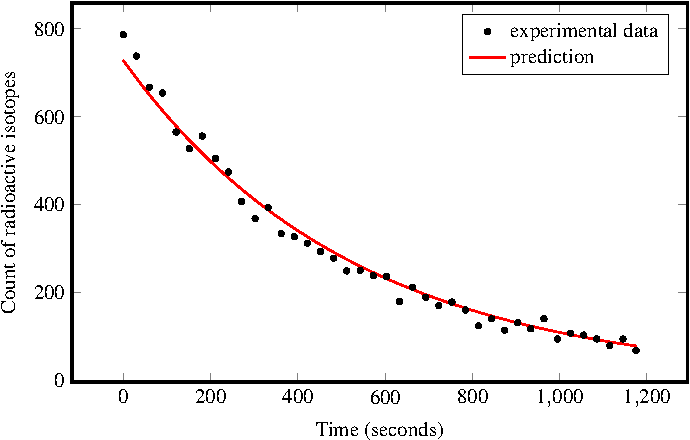
\includegraphics[scale=1.1]{image/12/copper-decay.pdf}
\caption{%%
  The radioactive decay of a sample of copper that had been neutron
  activated.  The black dots show the experimental data from
  \Table{tab:logarithm:copper_radioactive_decay} and the red curve is
  a graph of \Equation{eqn:logarithm:copper_decay_model}.
}
\label{fig:logarithm:copper_decay_data_versus_prediction}
\end{figure}

\solutionpart{subex:logarithm:copper_decay_regression}
\Table{tab:logarithm:copper_decay_regression} shows the detailed
calculation for the linear regression model
$\ln Q(x) = rx + \ln a$.  From the table, you have the sums
\[
\sum_{i=1}^n (x_i - \xbar) (y_i - \ybar)
\approx
-9417.8213
%%
\qquad
\text{and}
\qquad
%%
\sum_{i=1}^n (x_i - \xbar)^2
\approx
4840149.975
\]
where $n = 40$ is the number of data points in the table.  Then $r$
and $\ln a$ can be estimated as
\[
r
\approx
-0.0019
%%
\qquad
\text{and}
\qquad
%%
\ln a
\approx
6.5903
\]
and hence the parameter $a$ can be estimated as
$a \approx 727.9879$, with both $r$ and $a$ rounded to four decimal
places.  If $Q(x)$ represents the number of remaining radioactive
isotopes in the sample of copper after $x$ seconds, then the data in
\Table{tab:logarithm:copper_radioactive_decay} can be modelled as the
exponential decay function
%%
\begin{equation}
\label{eqn:logarithm:copper_decay_model}
Q(x)
=
727.9879 \cdot e^{-0.0019 x}.
\end{equation}
%%
\Figure{fig:logarithm:copper_decay_data_versus_prediction} shows a
graph of \Equation{eqn:logarithm:copper_decay_model} together with a
scatter plot of the data from
\Table{tab:logarithm:copper_radioactive_decay}.

\solutionpart{subex:logarithm:copper_decay_RMS_error_Pearson_rho}
The model in \Equation{eqn:logarithm:copper_decay_model} has a root
mean square~(RMS) error of $22.7376$, rounded to four decimal places.
Furthermore, the model has a Pearson correlation coefficient of
$\rho \approx -0.9924$, also rounded to four decimal places.  The low
values of the RMS error and $\rho$ suggest that
\Equation{eqn:logarithm:copper_decay_model} is a good fit of the
experimental data.
\end{solution}
}{}


%%%%%%%%%%%%%%%%%%%%%%%%%%%%%%%%%%%%%%%%%%%%%%%%%%%%%%%%%%%%%%%%%%%%%%%%%%%

\subsection{Logarithmic on horizontal axis}


%%%%%%%%%%%%%%%%%%%%%%%%%%%%%%%%%%%%%%%%%%%%%%%%%%%%%%%%%%%%%%%%%%%%%%%%%%%

\subsection{Logarithmic on both axes}

As an example, \Figure{fig:logarithm:Fortune100} shows two scatter
plots of the same data set on the number of employees and revenue of
the top $100$ companies in the USA.\footnote{
  The data set was available at:
  \url{http://fortune.com/fortune500/list/},
  accessed 2018-05-13.
}
Note that the scatter plot in \Figure{fig:logarithm:Fortune100_linear}
has the usual linear scale for the horizontal and vertical axes.  Up
to now, you have been producing scatter plots with linear scaling.  In
its present form, the scatter plot shows a cluster of points in the
lower-left corner and one point in the upper-right corner.  What about
the spacing of the points in the cluster?  Suppose you take the
logarithm to base $10$ of each number on the horizontal and vertical
axes.  The result is the scatter plot in
\Figure{fig:logarithm:Fortune100_log}, which clearly shows the spacing
of the points in terms of multiples of $10$.  The graph in
\Figure{fig:logarithm:Fortune100_log} is called a \emph{log-log} plot
because numbers on both the horizontal and vertical axes have been
transformed to their equivalents under the common logarithm.

\begin{figure}[!htbp]
\centering
\subfigure[]{
  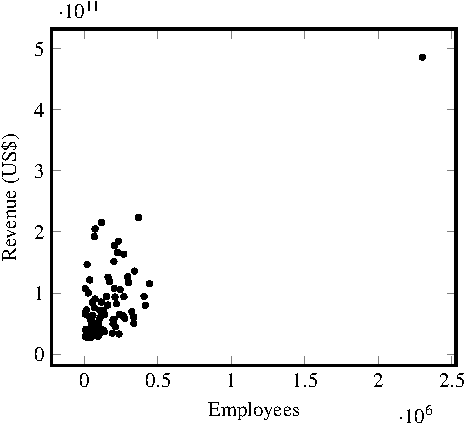
\includegraphics[scale=0.8]{image/12/fortune100-linear.pdf}
  \label{fig:logarithm:Fortune100_linear}
}
%%
%%
\subfigure[]{
  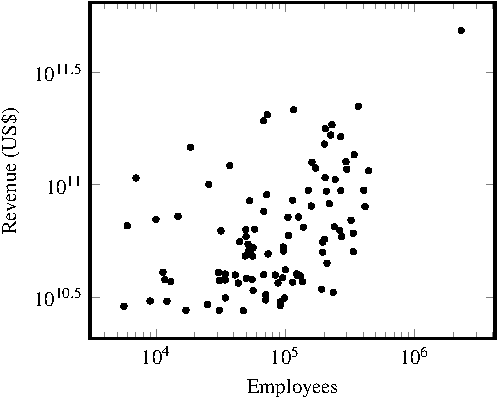
\includegraphics[scale=0.8]{image/12/fortune100-log.pdf}
  \label{fig:logarithm:Fortune100_log}
}
\caption{%%
  The number of employees versus the revenue of the top $100$ US
  companies.  Revenue is in US dollars.  (a)~A scatter plot with
  linear axes.  Each value on the horizontal and vertical axes should
  be multiplied by, respectively, $10^6$ and $10^{11}$.  (b)~A scatter
  plot with log-log axes.
}
\label{fig:logarithm:Fortune100}
\end{figure}


\newpage
%%%%%%%%%%%%%%%%%%%%%%%%%%%%%%%%%%%%%%%%%%%%%%%%%%%%%%%%%%%%%%%%%%%%%%%%%%%

\section*{Problem}

\begin{problem}
\item Read the following article by Kathleen M. Clark and Clemency
  Montelle:
  \emph{Logarithms: The Early History of a Familiar Function}.\footnote{
    The article is available at the website
    \url{http://web.archive.org/web/20180509072424/https://www.maa.org/press/periodicals/convergence/logarithms-the-early-history-of-a-familiar-function},
    accessed 2018-05-09.
  }

\item Exponential distribution and cricket.
\ifbool{showSolution}{
\begin{solution}

\end{solution}
}{}

\item Pressure and density above sea level.
\ifbool{showSolution}{
\begin{solution}

\end{solution}
}{}

\item Why can't the base be $b = 1$?
\ifbool{showSolution}{
\begin{solution}

\end{solution}
}{}

\item Prove the half-life formula for radioactive decay.  Derive the
  rule of $69$ for the half-life of an exponential decay model.
\ifbool{showSolution}{
\begin{solution}

\end{solution}
}{}

\item Prove the doubling-time formula for an exponential growth
  model.
\ifbool{showSolution}{
\begin{solution}

\end{solution}
}{}

\item Newton's law of cooling to determine when someone died.
\ifbool{showSolution}{
\begin{solution}

\end{solution}
}{}

\item Use the data set at:
  \url{http://resources.seattlecentral.edu/qelp/sets/071/071.html}
\ifbool{showSolution}{
\begin{solution}

\end{solution}
}{}

\item The Preston curve on GDP per capita versus life expectancy at
  birth.
\ifbool{showSolution}{
\begin{solution}

\end{solution}
}{}

\item Historical statistics on supply and demand of copper.\footnote{
    See the website:
    \url{https://minerals.usgs.gov/minerals/pubs/historical-statistics/},
    accessed 2018-05-15.
  }
\ifbool{showSolution}{
\begin{solution}

\end{solution}
}{}
\end{problem}

\end{document}
